% *********************************************************************
% © 2021–2026 Jeremy Sylvestre
%
% Permission is granted to copy, distribute and/or modify this document
% under the terms of the GNU Free Documentation License, Version 1.3 or
% any later version published by the Free Software Foundation; with no
% Invariant Sections, no Front-Cover Texts, and no Back-Cover Texts. A
% copy of the license is included in the appendix entitled “GNU Free
% Documentation License” that appears in the output document of this
% PreTeXt source code. All trademarks™ are the registered® marks of
% their respective owners.
%
% *********************************************************************

\newcommand*{\xmin}{-0.5}
\newcommand*{\xmax}{10}
\newcommand*{\ymin}{-0.25}
\newcommand*{\ymax}{1}

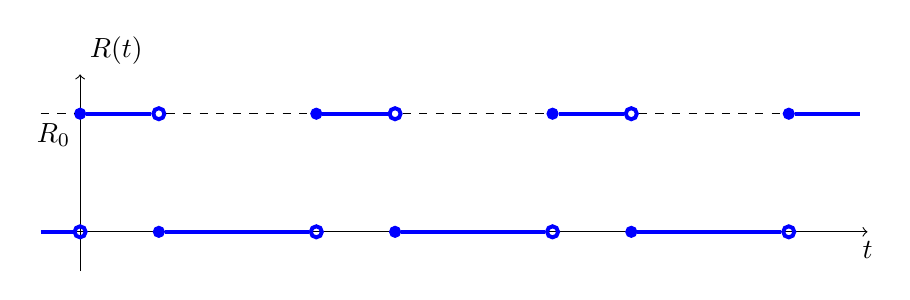
\begin{tikzpicture}
[
	closedpt/.style={circle,draw,fill,inner sep=0pt,minimum size=4pt},
	openpt/.style={circle,draw,inner sep=0pt,minimum size=4pt},
	yscale=2
]

	\node[below left] at (0,0.75) {$R_0$};

	% axes
	\draw[->,thin] (\xmin,0) -- (\xmax,0) node[below] {$t$};
	\draw[->,thin] (0,\ymin) -- (0,\ymax) node[above right] {$R(t)$};

	% off
	\node[blue,line width=0.5mm,openpt] at (0,0) (stop) {};
	\draw[blue,line width=0.5mm] (\xmin,0) -- (stop);

	% on
	\node[blue,closedpt] at (0,0.75) (onstart) {};
	\node[blue,line width=0.5mm,openpt] at (1,0.75) (onstop) {};
	\draw[blue,line width=0.5mm] (onstart) -- (onstop);
	\draw[dashed,thin] (\xmin,0.75) -- (onstart);

	% off
	\node[blue,closedpt] at (1,0) (start) {};
	\node[blue,line width=0.5mm,openpt] at (3,0) (stop) {};
	\draw[blue,line width=0.5mm] (start) -- (stop);

	% on
	\node[blue,closedpt] at (3,0.75) (onstart) {};
	\draw[dashed,thin] (onstop) -- (onstart);
	\node[blue,line width=0.5mm,openpt] at (4,0.75) (onstop) {};
	\draw[blue,line width=0.5mm] (onstart) -- (onstop);

	% off
	\node[blue,closedpt] at (4,0) (start) {};
	\node[blue,line width=0.5mm,openpt] at (6,0) (stop) {};
	\draw[blue,line width=0.5mm] (start) -- (stop);

	% on
	\node[blue,closedpt] at (6,0.75) (onstart) {};
	\draw[dashed,thin] (onstop) -- (onstart);
	\node[blue,line width=0.5mm,openpt] at (7,0.75) (onstop) {};
	\draw[blue,line width=0.5mm] (onstart) -- (onstop);

	% off
	\node[blue,closedpt] at (7,0) (start) {};
	\node[blue,line width=0.5mm,openpt] at (9,0) (stop) {};
	\draw[blue,line width=0.5mm] (start) -- (stop);

	% on
	\node[blue,closedpt] at (9,0.75) (onstart) {};
	\draw[dashed,thin] (onstop) -- (onstart);
	\draw[blue,line width=0.5mm] (onstart) -- (9.9,0.75);

\end{tikzpicture}
